\section{Inhalt der Vorlesung}
\begin{itemize}
	\item Logik: Aussagenlogik , Beweise
	\item Mengenlehre: Alle Objekte
	\item Kombinatorik
	\item Graphentheorie
	\item Zahlentheorie, Algebra
	\begin{itemize}
		\item Anwendungen: Kommunikation, Kryptologie, Fehlerkorrektur
	\end{itemize}
\end{itemize}

\chapter{Motivation}
\subsubsection{Worum geht es in dieser Vorlesung?}

\begin{bsp}[note = Modellierung]
\colorbox{White}{\parbox{3\skak}{
	\WhiteKnightOnBlack\WhiteEmptySquare\WhiteKnightOnBlack\\
	\WhiteEmptySquare\BlackEmptySquare\WhiteEmptySquare\\
	\BlackKnightOnBlack\WhiteEmptySquare\BlackKnightOnBlack
}} $\longrightarrow$
\colorbox{White}{\parbox{3\skak}{
	\WhiteKnightOnBlack\WhiteEmptySquare\BlackKnightOnBlack\\
	\WhiteEmptySquare\BlackEmptySquare\WhiteEmptySquare\\
	\BlackKnightOnBlack\WhiteEmptySquare\WhiteKnightOnBlack
}}\\
BILD \\
Fazit: \\
\begin{itemize}
	\item Wegschälen vom Umweltlichen hat das Problem einfach gemacht $\implies$ \textbf{Abbstraktion}
	\item Viele diskrete Probleme führen auf Graphen
\end{itemize}
\end{bsp}

\begin{bsp}[note = Zahlentheorie]
	\begin{gather*}
		N = \{ 0 , 1 , 2 , 3 , \ldots \} \\
 		a \mid b \qquad \text{\enquote{a teil b}} \qquad a , b \in \mathbb{N} \\
		a \mid b :\leftrightarrow \exists n \in \mathbb{N} : a \cdot n = b
	\end{gather*}

	\begin{bsp*}
		\begin{gather*}
			2 \mid 6 \\
			3 \nmid 6 \\
			2 \equiv 5 \pmod 3 \\
			3 \not\equiv 5 \pmod 3
		\end{gather*}
	\end{bsp*}
	\begin{equation*}
		\text{p Primzahl} :\leftrightarrow ( a \mid p \rightarrow ( a = 1 \vee a = p ) \wedge p \neq 1 )
	\end{equation*}
	\textbf{Intuition} $\leftrightarrow$ \textbf{Beweis}

	Jede Zahl hat eine \textbf{eindeutige} Primzahlzerlegung (nämlich: \[ p \mid (a \cdot b) \rightarrow p \mid a \vee p \mid b \quad ; \] wir haben's noch nicht bewiesen) \\
	\begin{satz*}
		Es gibt unendlich viele Primzahlen
		\begin{bew}[note = Euklid]
			Annahme: Es gibt nur endlich viele Primzahlen $p_1 , \ldots , p_n$
			\begin{gather*}
				M = p_1 \cdot p_2 \cdot \dotsm \cdot p_n + 1 \\
				\forall i : p_i \nmid M \\
				\text{\lightning} \: \blacksquare
			\end{gather*}
		\end{bew}
	\end{satz*}
\end{bsp}

\begin{bsp}[note = Kombinatorik (\enquote{systematisches Zählen})]
	Kette mit $p$ Perlen in $a$ verschiedene Farben \\
	Anzahl mögliche Ketten? $a^n$ \\
	Anzahl Muster? \\
	Wie oft kommt jedes Muster vor? \\
	Gegeben: $p$ ist prim \\
	\begin{tabular}{ l l }
	$\implies$ einfärbig:		& 1 mal \\
	$\implies$ mehrfärbig:	& p mal
	\end{tabular}
	\begin{gather*}
		\implies \frac{a^p - a}{p} + a = a \cdot ( 1 + \frac{a^{p-1} - 1}{p} ) \\
		a \text{ beliebig}, p \text{ Primzahl} \\
		p \mid ( a^p - a ) \\
		a^p \equiv a \pmod p \\
		( p \nmid a ) \rightarrow ( a^{p-1} \equiv 1 \pmod p ) \\
		\textbf{Kleines Satz von Fermat}
	\end{gather*}
\end{bsp}

\begin{bsp}[note = Geometrie]
	Rechteckige Terrase $a \cdot b \mid a,b \in \mathbb{N}$ \\
	Was sind die grösstmöglichen Quadratplatten, mit denen mann sie exakt belegen kann? \\
	$a \geq b$ \quad Quardat aufteilen in $b \cdot b$ und $(a-b) \cdot b$ \\
	Beobachtungen:
	\begin{itemize}
		\item Jede Belegung des ganzen führt auf separate Belegungen von \\$[b \cdot b]$ und $[(a-b) \cdot b]$
		\item Es reicht, $[(a-b) \cdot b]$ zu berechnen.
	\end{itemize}
	$$\mathrm{R}_{a-b}(b) = b \bmod (a-b)$$
	Fortfahren, bis wir ein Quadrat erhalten. Warum wird das sicher passieren? \\
	\quad Spätestens bei $1 \cdot 1$\\
	Algorithmus (Euklid):
	\begin{gather*}
		a , b \\
		r_1 = \mathrm{R}_b(a) \\
		r_2 = \mathrm{R}_{r_1}(b) \\
		\vdots \\
		r_n = \mathrm{R}_{r_{n-1}}(r_{n-2}) \\
		\vdots \\
		r_k = \ggt(a,b) \\
		0
	\end{gather*}
\end{bsp}

\begin{bsp}
	2 Sanuhren: 21 min und 15 min. Wir wollen 3 min abmessen. \\
	\begin{tabular}{ c c c c c c }
		Euklid:	& 21,	& 15,	& 6,	& 3,	& 0 \\
		21 min:	& 1	&0	&1	&-2 \\
		15 min:	&0	&1	& -1	&3
	\end{tabular}
\end{bsp}

\begin{bsp}[note = Verbindungen ohne Überkreuzen]
	3 Häuser mit 3 Werke verbinden $\rightarrow$ geht nicht! \\
	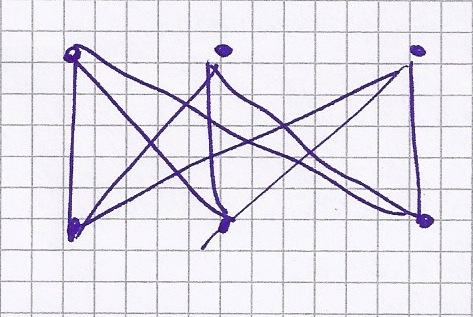
\includegraphics{Bild2} \\
	der Graph ist nicht \textbf{planar}. \\
	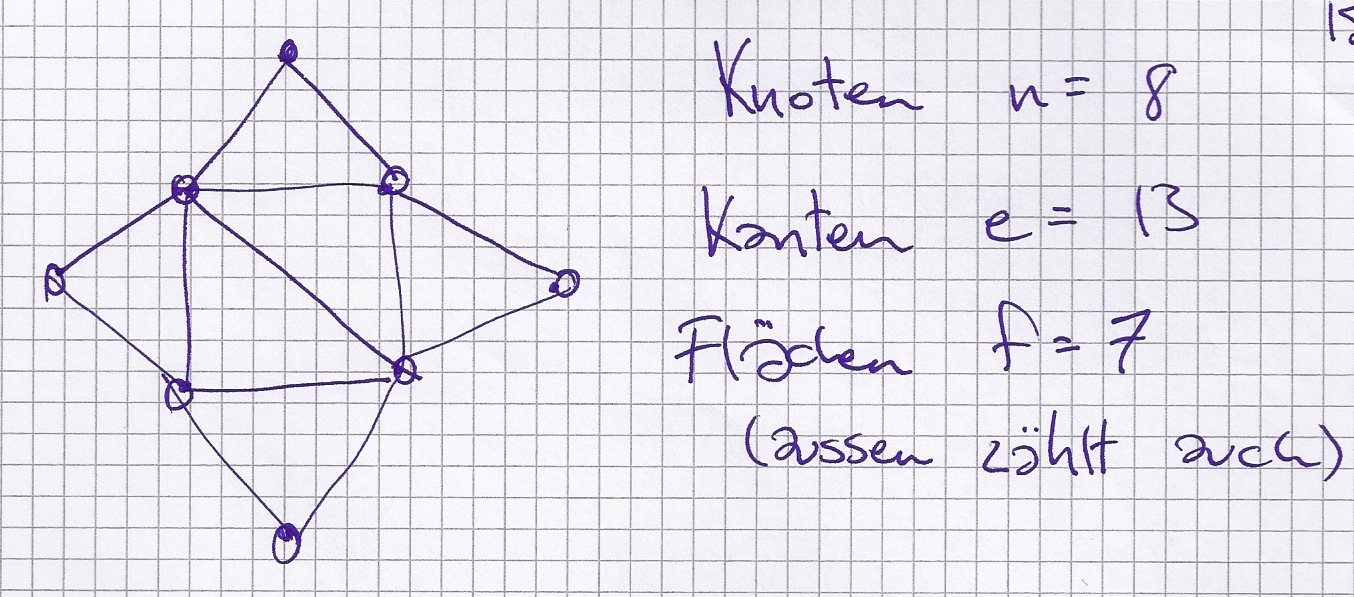
\includegraphics[width=\textwidth]{Bild3}
	\begin{bew}[head = Beweisidee:]
		\quad Für einen Baum (kreislos, zusammenhängend) gilt $n = e +1 \implies n - e + f = 2$ \\
		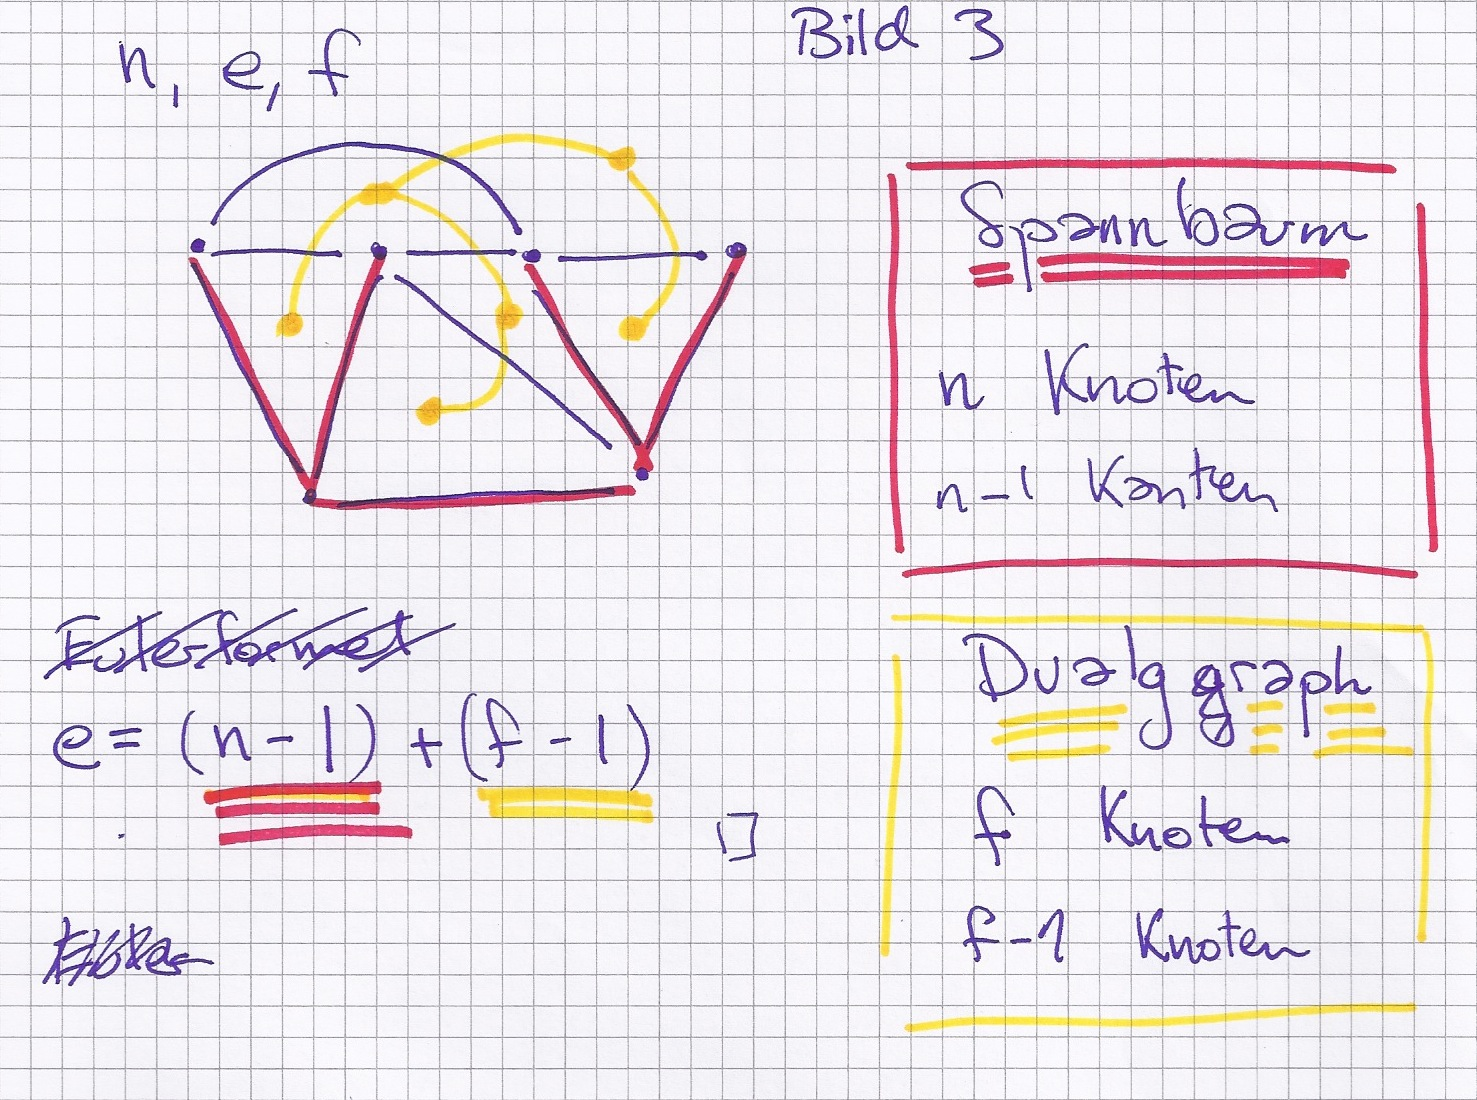
\includegraphics[width=\textwidth]{Bild4} \\
		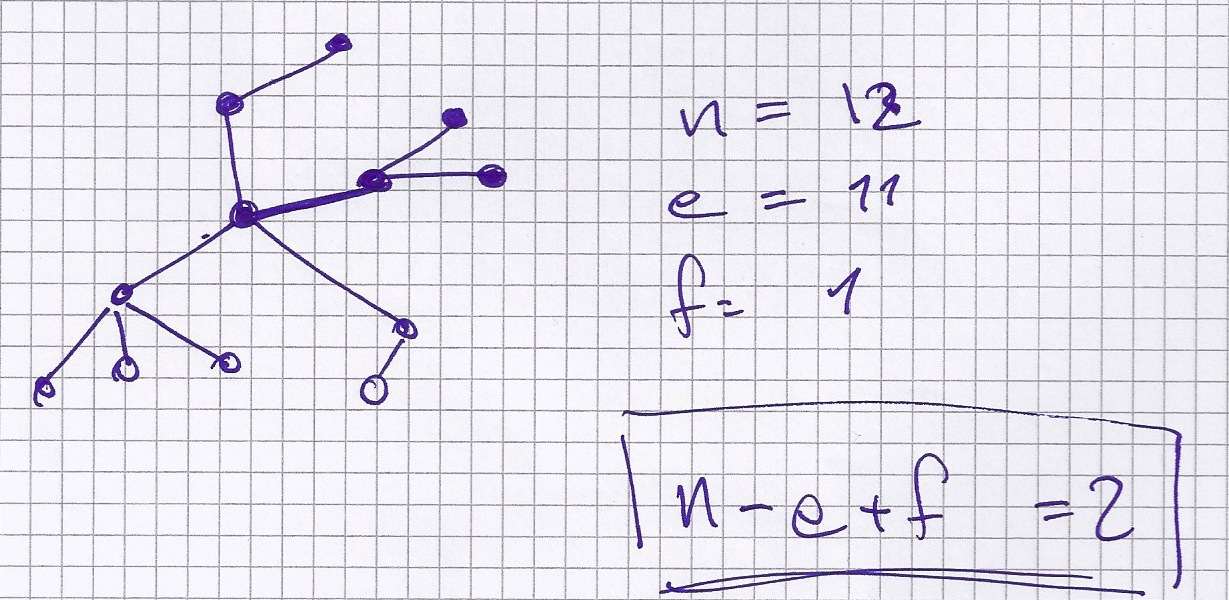
\includegraphics[width=\textwidth]{Bild5} \\
		\textbf{Eulersche Polyederformel}
	\end{bew}
\end{bsp}
